\documentclass{article}

\usepackage{graphicx}
\usepackage{tikz}
\usepackage{tikzsymbols}
\usetikzlibrary{calc,patterns,shapes.geometric}
\pagestyle{empty}
\usepackage[margin=0pt]{geometry}
\geometry{papersize={14in,12in}}

\def\centerarc[#1](#2)(#3:#4:#5){\draw[#1] ($(#2)+({#5*cos(#3)},{#5*sin(#3)})$) arc (#3:#4:#5);}

\begin{document}
	\begin{figure}
		\centering
		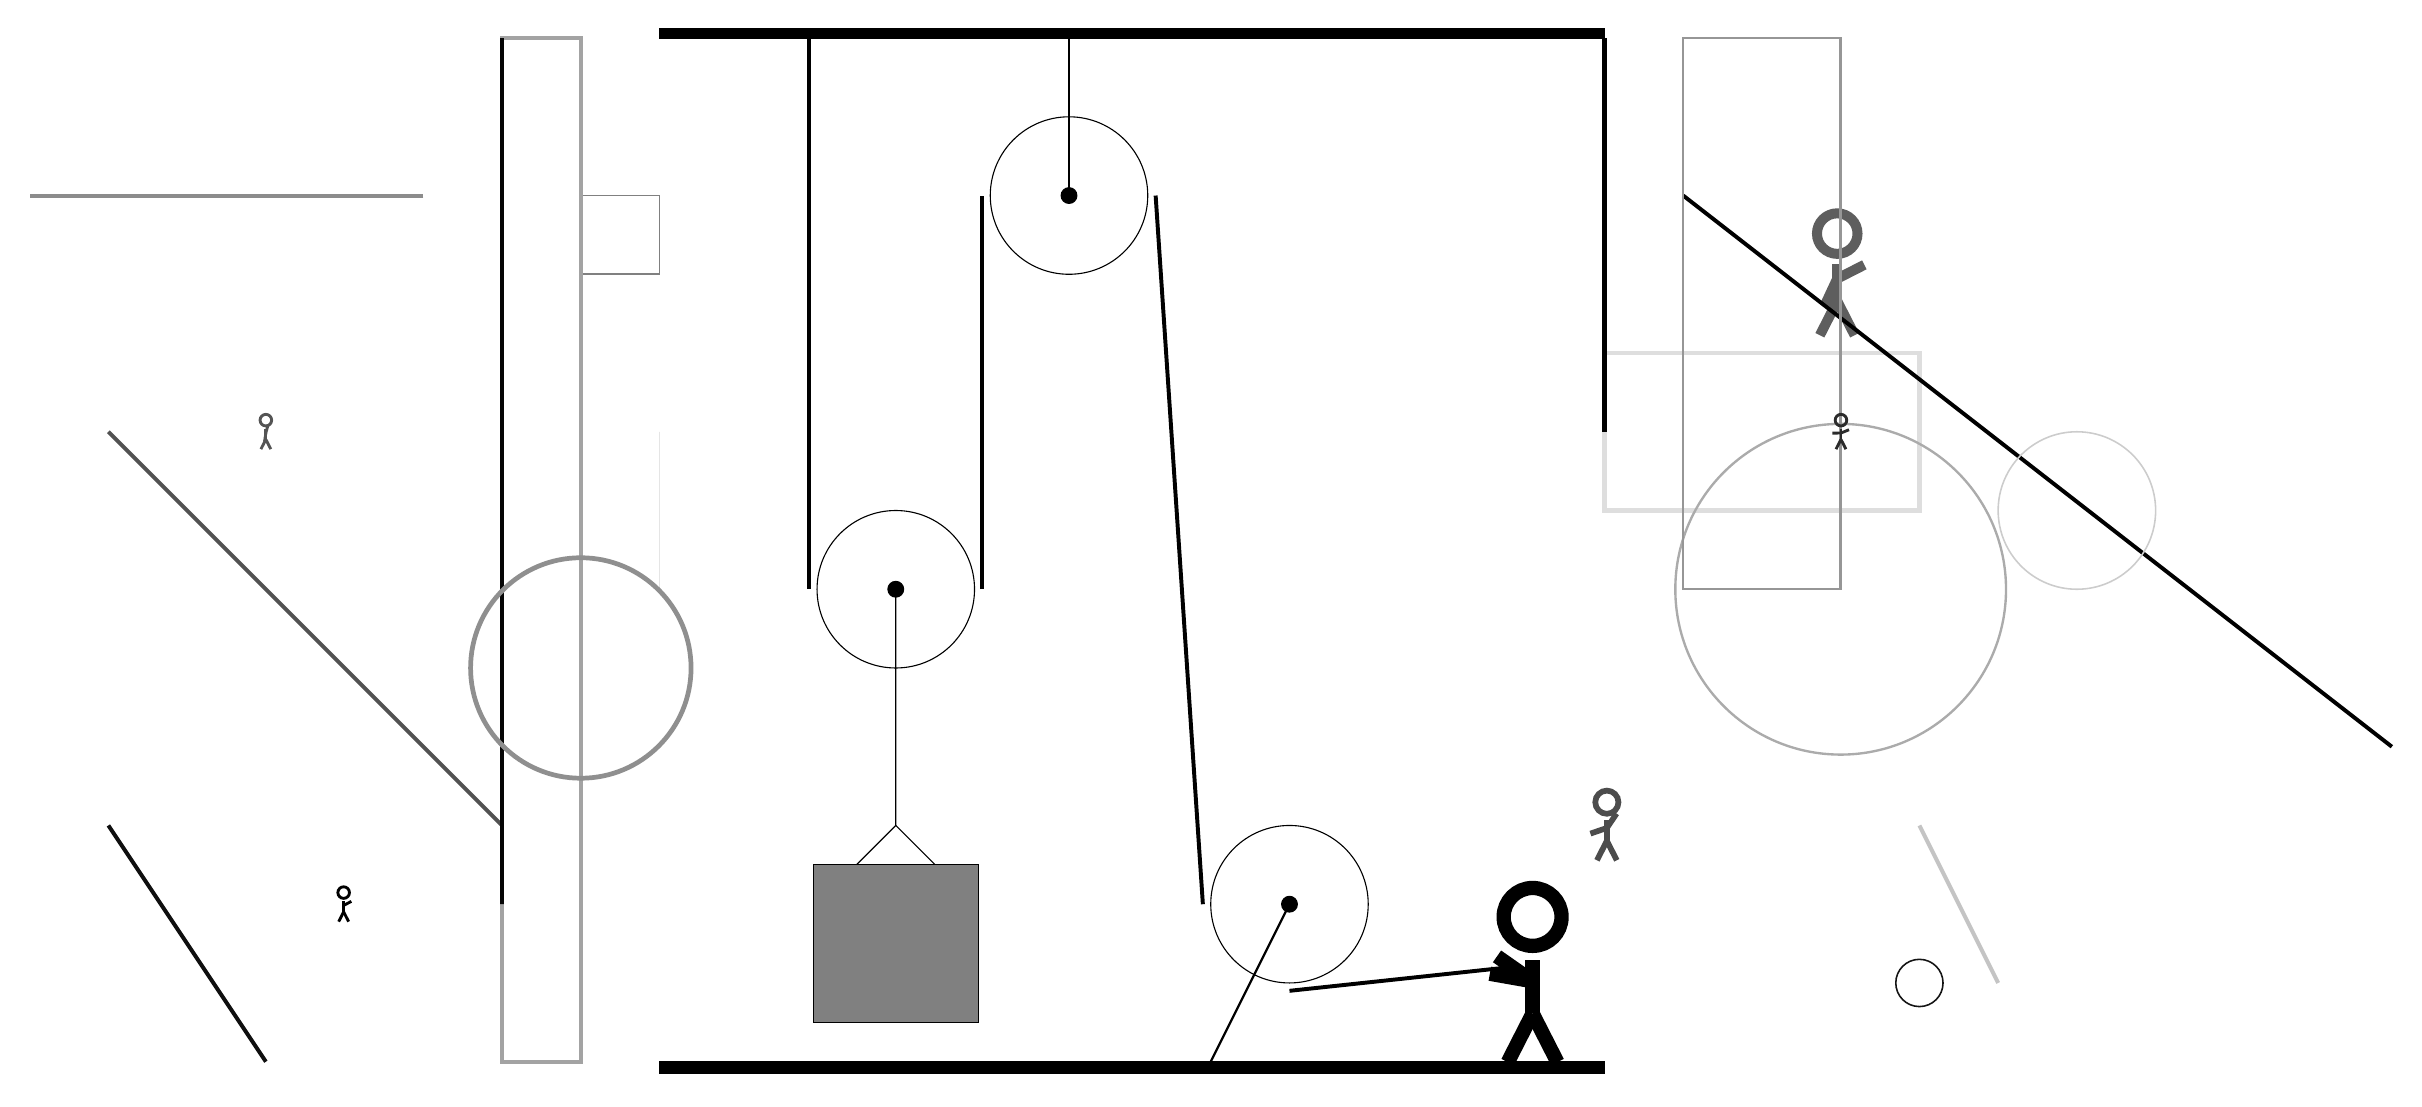
\begin{tikzpicture}
			%%%%% START %%%%%
			
			\draw[fill=black] (-2, 10) rectangle (10, 10.125);
			
			\draw (3.2, 8.0) circle (1);
			\draw[fill=black] (3.2, 8.0) circle (0.1);
			\draw[thick] (3.2, 8.0) -- (3.2, 10);
			
			\draw (6, -1) circle (1);
			\draw[fill=black] (6, -1) circle (0.1);
			\draw[thick] (6, -1) -- (5, -3);
			
			\draw (1, 3.0) circle (1);
			\draw[fill=black] (1, 3.0) circle (0.1);
			
			\draw (1, 3.0) -- (1, 0) -- (0.5, -0.5);
			\draw (1, 0) -- (1.5, -0.5);
			\draw[fill=black!50] (-0.05, -0.5) rectangle (2.05, -2.5);
			
			\draw[line width=0.5mm] (-0.1, 10) -- (-0.1, 3.0);
			\centerarc[line width=0.5mm](1, 3.0)(180:360:1.1);
			\draw[line width=0.5mm](2.1, 3.0) -- (2.1, 8.0);
			\centerarc[line width=0.5mm](3.2, 8.0)(0:180:1.1);
			\draw[line width=0.5mm](4.3, 8.0) -- (4.9, -1);
			\centerarc[line width=0.5mm](6, -1)(180:270:1.1);
			\draw[line width=0.5mm](6, -2.1) -- (8.8, -1.8);
			
			\draw[line width=0.5mm, color=black!23](14, 0) -- (15, -2);
			
			\draw[line width=0.6mm, color=black!13] (10, 4) rectangle (14, 6);
			\node[line width=0.3mm, color=black!100] at (-6, -1) {\Strichmaxerl[2][90][28]};
			\draw[line width=0.5mm, color=black!45](-5, 8) -- (-10, 8);
			\draw [line width=0.3mm, color=black!33](13, 3) circle (2.1);
			
			\draw [line width=0.2mm, color=black!92](14, -2) circle (0.3);
			
			\draw[line width=0.2mm, color=black!50] (-2, 8) rectangle (-3, 7);
			
			\draw[line width=0.2mm, color=black!10] (-2, 3) rectangle (-2, 5);
			\draw[line width=0.5mm, color=black!36] (-4, -3) rectangle (-3, 10);
			\node[line width=0.3mm, color=black!63] at (13, 7) {\Strichmaxerl[7][65][27]};
			\draw[line width=0.5mm, color=black!100](11, 8) -- (20, 1);
			\draw[line width=0.5mm, color=black!94](-7, -3) -- (-9, 0);
			\draw[line width=0.5mm, color=black!68](-4, 0) -- (-9, 5);
			
			\node[line width=0.3mm, color=black!67] at (-7, 5) {\Strichmaxerl[2][81][75]};
			\node[line width=0.6mm, color=black!70] at (10, 0) {\Strichmaxerl[4][19][56]};
			\draw[line width=0.3mm, color=black!41] (11, 3) rectangle (13, 10);
			\node[line width=0.6mm, color=black!83] at (13, 5) {\Strichmaxerl[2][1][22]};
			
			\draw[line width=0.6mm, color=black!98] (-4, 10) rectangle (-4, -1);
			\draw [line width=0.2mm, color=black!20](16, 4) circle (1.0);
			
			\draw[line width=0.6mm, color=black!100] (10, 10) rectangle (10, 5);
			\draw [line width=0.6mm, color=black!44](-3, 2) circle (1.4);
			
			
			\node at (9, -1.9) {\Strichmaxerl[10][-35][170]};
			
			\draw[fill=black] (-2, -3) rectangle (10, -3.15);
			
			%%%%% END %%%%%
		\end{tikzpicture}
	\end{figure}	
\end{document}